\documentclass[graybox]{svmult}

\usepackage{amssymb}
\usepackage{graphicx}
\usepackage{caption}
\usepackage{subcaption}
\usepackage[colorlinks,linkcolor=blue]{hyperref}
\usepackage{todonotes}
\usepackage{type1cm}
\usepackage{makeidx}
\usepackage{graphicx}
\usepackage{multicol}
\usepackage[bottom]{footmisc}
\usepackage{newtxtext}
\usepackage[varvw]{newtxmath}
\usepackage{wrapfig}

\makeindex

\begin{document}

\title*{A discrete event formalism for fast simulation of on-demand transportation systems}

%\author{Anonymous Author and Anonymous Author}
\author{Dominik Ascher and Georg Hackenberg}

%\institute{
%	Anonymous Author
%	\at
%	Reserved for author affiliation
%	\and
%	Anonymous Author
%	\at
%	Reserved for author affiliation
%}

%\institute{
%    Dominik Ascher
%    \at
%    Distributed Artificial Intelligence Laboratory, Faculty of Electrical Engineering and Computer Science, Technical University of Berlin, 10587 Berlin, Germany, \email{ascher@tu-berlin.de}
%    \and
%    Georg Hackenberg
%    \at
%    School of Engineering, University of Applied Sciences Upper Austria, 4600 Wels, Austria, \email{georg.hackenberg@fh-wels.at}
%}

\maketitle

\abstract{
	The interconnection between intelligent transportation systems (ITS) and services poses fundamental challenges with respect to establishing most efficient structures, infrastructures, as well as intelligent and integrated control strategies addressing new transportation paradigms such as autonomous vehicles, mobility-on-demand as well as the transportation electrification. Systematic methods for efficiently modeling, simulating and evaluating these systems are required, which are able to address aforementioned challenges.
	For this, we present a formalization of essential static properties, dynamic state functions, as well as events concisely describing transportation system design space in the scope of emerging transportation paradigms. Our proposed formalization allows for reduction of simulation complexity by focusing on relevant events impacting the design problem at hand only, while omitting unimportant details negatively impacting simulation performance, thereby reducing both modeling as well as simulation effort. In addition, the provided formalization of system theory and discrete events serves as an interface for deriving well-defined system structure as well as efficient control strategies. 
}

\section{Introduction}
\label{sec:intro}

Emerging transportation paradigms such as autonomous vehicles \cite{hancock2019future}, mobility-on-demand \cite{atasoy2015concept} and the transportation electrification \cite{pereirinha2018main} are fundamental drivers for the increasing transformation of current transportation systems. As these paradigms are crucial for addressing 21st century challenges such as meeting sustainability goals and reducing carbon emissions \cite{sachs2019six}, their efficient integration, such as in the context of shared and autonomous vehicles \cite{narayanan2020shared}, represents a key challenge for establishing intelligent transportation systems (ITS) \cite{figueiredo2001towards}. To derive most efficient transportation system designs and control strategies for the latter, as well as to project relevant scenarios of utilizing them, wholistic and integrated systems engineering techniques for modeling and evaluating according system design options are required.
Here, modeling and simulation based systems engineering \cite{gianni2014modeling} is widely used for tasks such as analysis, design and decision making with respect to systems engineering processes, where simulation aids projecting and obtaining information about system under design and environment behavior.
However, as simulation complexity increases with the number and dimensionality of considered parameters, states and actions of modeled systems, simulation accuracy decreases with simplifying model assumptions as well as discretization of states and time, thereby limiting system model expresiveness or approximation accuracy, i.e. validity, to a defined level of abstraction.
Here, Discrete-Event Simulation (DES) \cite{fishman2001discrete} represents a generic formalism, applicable to the considered integrated system problem incorporating aforementioned emerging transportation paradigms, which significantly reduces simulation complexity by limiting action space dimensionality and by abstracting from discrete-time resolutions through the use of events. For this, events are defined as functions over a systems trajectory of states, which precisely indicate when actions needs to be taken. 

\subsection{Related work}
In recent years, DES has seen increased research attention in the transportation domain, especially with respect to applications for autonomous vehicles, electric vehicles and their charging behavior, as well as shared mobility, and, finally, in contexts combining the former.

For the transportation domain context in general (e.g. \cite{burghout2006discrete}), DES can be used to formalize the the behavior of vehicles in terms of their movements within any given infrastructure described by a transport network. Then, based on this, in applications of DES in a shared mobility context (e.g. \cite{clemente2013discrete}) a fleet of vehicles is shared and utilized among a set of passengers driving from origin, i.e. pick-up, to destination, i.e. drop-off, positions. Futhermore, in this context, autonomous vehicles may be incorporated, where a supply of autonomous vehicles covers the demands of passengers instead, thereby typically assuming the form of autonomous mobility-on-demand systems (e.g. \cite{jager2018multi, gurumurthy2021system}).
Then, with respect to DES applied in the context of modeling electric vehicles and their charging behavior, existing approaches focus on describing behavior between electric vehicles and charging stations (e.g. \cite{lebeau2013implementing}), or on investigating home charging behavior of electric vehicles of private users (e.g.~\cite{lopez2021modeling}), or to assess interactions arising from electric vehicle charging on the power grid (e.g.  \cite{darabi2013event, ferro2019predictive}).
Finally, in approaches where DES is applied in contexts combining the former concepts, i.e. where electric vehicles enable shared mobility services, electric vehicles are utilized by drivers through carsharing services (e.g. \cite{fanti2017fleet, hamroun2020modelling, li2021simulation}), where models aim to assess the combined interactions resulting from aforementioned concepts.

\subsection{Problem statement}

Simulation complexity of integrated systems rises according to model complexity, such as number, dimensionality and discretization of system states and actions. While DES helps decreasing simulation complexity, current approaches for modeling, simulating and evaluating transportation system designs are not able to address integrated system problems holistically incorporating new transportation paradigms.
Therefore, to establish concise models and efficient simulations of these integrated systems, we consider it crucial to determine a required set of essential system properties, dynamic state functions as well as events, which are necessary and relevant for describing integrated system problems in the context of emerging transportation paradigms such as autonomous vehicles, mobility-on-demand and the transportation electrification.

\subsection{Contribution}
To address this situation, in this work, we provide a discrete-event formalism for fast simulation of on-demand transportation systems.
For this, in Section~\ref{sec:theory} we provide a formalization of the underlying system theory of our approach, which focuses on definition of a concise and essential set of static properties and dynamic states for establishing models of transportation systems in the context of autonomous vehicles, mobility-on-demand and the transportation electrification.
Then, in Section~\ref{sec:events}, based on introduced system theory, we provide a formalization of discrete events for determining decisions that must be considered for high-performance state computation, where event-based formalization supports abstraction and complexity reduction of both system modeling and simulation, and can be utilized for deriving well-defined and efficient control strategies. 
Finally, in Section~\ref{sec:con}, we conclude with a short discussion of our approach as well as its application for deriving system designs and control strategies, and provide an outlook.

\section{System theory}
\label{sec:theory}

The system theory presented in this work is intended to capture a concise and an essential set of static properties, static calculations, and dynamic states for establishing sound models and control strategies for on-demand transportation systems.
These static properties, static calculations, and dynamic states serve as a foundation for further abstraction and reduction of system simulation complexity using discrete events, for which we refer to Section~\ref{sec:events}.

\begin{figure}[htbp]
	\centering
	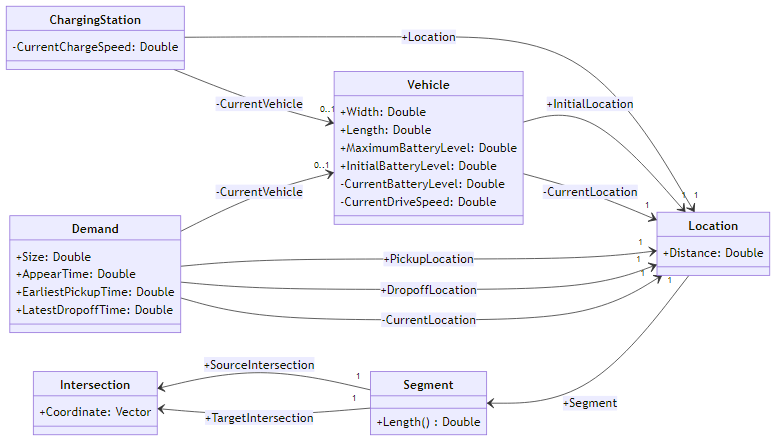
\includegraphics[width=\textwidth]{../../diagrams/model/classes-v0.1.png}
	\caption{Concepts in the class diagram notation of the Unified Modeling Language (UML), where \textit{public} UML attributes and relations represent \textit{static properties}, \textit{public} UML methods represents \textit{static calculations}, and \textit{private} UML attributes and relations represent \textit{dynamic states}.}
	\label{fig:concepts}
\end{figure}

Figure~\ref{fig:concepts} provides an overview of the proposed discrete event formalism.
We use intersections $i \in I$, segments $s \in S$ as well as locations $l \in L$ for describing properties about the transportation infrastructure.
Based on the transportation infrastructure, we use charging stations $cs \in CS$ for describing the charging infrastructure.
In addition, we describe transportation demands $d \in D$ on the transportation infrastructure. 
Finally, we use vehicles $v \in V$ for describing transportation supply and capacities.
In the following, we describe each concept in more detail including their static (i.e.\ time-independent) properties and calculations as well as their dynamic (i.e.\ time-dependent) state functions typically sampled during computer simulations.
We describe intersections, segments and locations in Section \ref{sec:intersections-segments}, and charging stations, demands as well as vehicles in Section \ref{sec:chargingstations-demands-vehicles}.

\subsection{Intersections, segments and locations}
\label{sec:intersections-segments}

In this Section, we describe intersections and segments of the transportation infrastructure as well as locations. These concepts are visualized in Figure \ref{fig:intersections-segments}.

\begin{figure}[htbp]
	\centering
	\begin{subfigure}{.2\textwidth}
		\centering
		
\includegraphics[scale=0.4]{../../concepts/intersection.png}
		\caption{Intersection}
		\label{fig:intersection}
	\end{subfigure}
	\begin{subfigure}{.35\textwidth}
		\centering
		
\includegraphics[scale=0.4]{../../concepts/segment.png}
		\caption{Segment}
		\label{fig:segment}
	\end{subfigure}
	\begin{subfigure}{.35\textwidth}
		\centering
		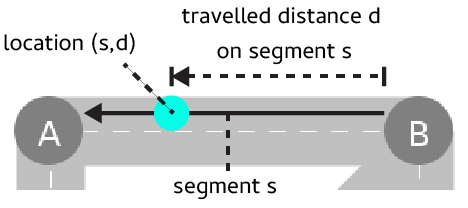
\includegraphics[scale=0.4]{../../concepts/location.png}
		\caption{Location}
		\label{fig:location}
	\end{subfigure}
	\caption{Intersections, segments and locations.}
	\label{fig:intersections-segments}	
\end{figure}

\vspace{2mm}

\noindent \textbf{Intersections} (see Figure \ref{fig:intersection}) define the routing points of the transportation infrastructure.
Each intersection must have a coordinate in the corresponding reference coordinate system such as the three-dimensional Euclidean space.
Mathematically, \textit{intersections} can be described as elements $i \in I$ with the following static property functions $P_{I}$:
\begin{itemize}
	\item $P_{I.C}: I \rightarrow \mathbb{R}^3$ represents the coordinate $c = P_{I.C}(i)$ of the intersection $i$ in coordinate system units.
\end{itemize}

\noindent \textbf{Segments} (see Figure \ref{fig:segment}) define the straight roads of the transportation infrastructure.
Each segment must define a source and a target intersection, which represent the start and the end coordinates of the straight road.
The length of the segment can be computed from the coordinates of the source and the target intersection.
Additionally, each segment must define a width and a maximum drive speed.
Mathematically, \textit{segments} can be described as elements $s = (i_s, i_t) \in I \times I = S$ with source intersection $i_s \in I$ and target intersection $i_t \in I$, such that the source intersection $i_s$ is not equal to the target intersection $i_t$, i.e.\ $i_s \neq i_t$.
Then, we define the following static calculation functions $C_{S}$:
\begin{itemize}
	\item $C_{S.L}: S \rightarrow \mathbb{R}_0^+$ represents the length $l = P_{S.L}(s)$ of segment $s$ in coordinate system units, such that the length $l$ equals to the Euclidean distance between the coordinate $c_s = P_{I.C}(i_s)$ of source intersection $i_s = P_{S.SI}(s)$ and coordinate $c_t = P_{I.C}(i_t)$ of target intersection $i_t = P_{S.TI}(s)$, i.e.\ $l = |c_t - c_s|$.
\end{itemize}

\noindent \textbf{Locations} (see Figure~\ref{fig:location}) define charging station, demand, and vehicle positions on the transportation infrastructure.
Each location must define a segment and a traveled distance on that segment.
Mathematically, \textit{locations} can be described as elements $l = (s, d) \in S \times \mathbb{R}_0^+ = L$ with segment $s$ and distance $d$ in coordinate system units, such that the distance $d$ is less than or equal to the length $l = C_{S.L}(s)$ of segment $s$, i.e.\ $d \leq l$.

\subsection{Charging stations, demands and vehicles}
\label{sec:chargingstations-demands-vehicles}

In this Section, we describe charging stations, demands as well as vehicles. These concepts are visualized in Figure \ref{fig:chargingstations-demands-vehicles}.

\begin{figure}[htbp]
	\centering
	\begin{subfigure}{.35\textwidth}
		\centering
		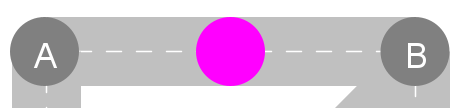
\includegraphics[scale=0.3]{../../concepts/charge-station.png}
		\caption{Charging station}
		\label{fig:charging-station}	
	\end{subfigure}
	\begin{subfigure}{.35\textwidth}
		\centering
		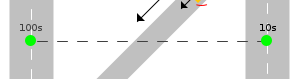
\includegraphics[scale=0.5]{../../concepts/demand.png}
		\caption{Demand}
		\label{fig:demand}
	\end{subfigure}
	\begin{subfigure}{.2\textwidth}
		\centering
		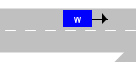
\includegraphics[scale=0.5]{../../concepts/vehicle.png}
		\caption{Vehicle}
		\label{fig:vehicle}	
	\end{subfigure}
	\caption{Charging stations, demands and vehicles.}
	\label{fig:chargingstations-demands-vehicles}	
\end{figure}

%\vspace{2mm}
\noindent \textbf{Charging stations} (see Figure \ref{fig:charging-station}) define locations on the transportation infrastructure, where vehicles can refill their batteries.
Mathematically, \textit{charging stations} can be described as elements $cs \in CS$ with the following static property functions $P_{CS}$:
\begin{itemize}
	\item $P_{CS.L}: CS \rightarrow L$ represents the location $l = P_{CS.L}(cs)$ of charging station $cs$.
\end{itemize}
For charging stations, computer simulations typically sample the following dynamic state functions $S_{CS}$:
\begin{itemize}
	\item $S_{CS.CV}: CS \times \mathbb{T} \rightarrow V \cup \{\perp\}$ represents the current vehicle $v = S_{CS.CV}(cs, t)$ connected to charging station $cs$ and time $t$, and
	\item $S_{CS.CCS}: CS \times \mathbb{T} \rightarrow \mathbb{R}^+$ represents the current charge speed $ccs = S_{CS.CCS}(cs, t)$ at charging station $cs$ and time $t$ in battery size units per time unit, such that the current charge speed $ccs$ is smaller than or equal to the maximum charge speed $mcs$, i.e.\ $ccs \leq mcs$.
\end{itemize}

\noindent \textbf{Demands} (see Figure \ref{fig:demand}) define the transportation loads that temporarily consume the available transportation capacities.
Mathematically, \textit{demands} can be described as elements $d \in D$ with the following static property functions $P_{D}$:
\begin{itemize}
	\item $P_{D.S}: D \rightarrow \mathbb{R}^+$ represents the size $s = P_{D.S}(d)$ of demand $d$ in demand size units,
	\item $P_{D.AT}: D \rightarrow \mathbb{T}$ represents the appearance time $at = P_{D.AT}(d)$ of demand $d$ in time units,
	\item $P_{D.EPT}: D \rightarrow \mathbb{T}$ represents the earliest pick-up time $ept = P_{D.EPT}(d)$ of demand $d$ in time units, such that the earliest pick-up time $ept$ is greater than or equal to the appearance time $at$, i.e.\ $ept \geq at$,
	\item $P_{D.LDT}: D \rightarrow \mathbb{T}$ represents the latest drop-off time $ldt = P_{D.LDT}(d)$ of demand $d$ in time units, such that the latest drop-off time $ldt$ is greater than the earliest pick-up time $ept$, i.e.\ $ldt > ept$,
	\item $P_{D.PL}: D \rightarrow L$ represents the pick-up location $pl = P_{D.PL}(d)$ of demand $d$, and
	\item $P_{D.DL}: D \rightarrow L$ represents the drop-off location $dl = P_{D.DL}(d)$ of demand $d$, such that the drop-off location $dl$ is not equal to the pick-up location $pl$, i.e.\ $dl \neq pl$.
\end{itemize}
For demands, computer simulations typically sample the following dynamic state functions $S_{D}$:
\begin{itemize}
	\item $S_{D.CV}: D \times \mathbb{T} \rightarrow V \cup \{\perp\}$ represents the current vehicle $v = S_{D.CV}(d, t)$ carrying demand $d$ at time $t$, and
	\item $S_{D.CL}: D \times \mathbb{T} \rightarrow L$ represents the current location $cl = S_{D.CL}(d, t)$ of demand $d$ at time $t$.
\end{itemize}

\noindent \textbf{Vehicles} (see Figure \ref{fig:vehicle})  define the transportation capacities available on the transportation infrastructure.
Mathematically, \textit{vehicles} can be described as elements $v \in V$ with the following static property functions $P_{V}$:
\begin{itemize}
	\item $P_{V.L}: V \rightarrow \mathbb{R}_0^+$ represents the length $l = P_{V.L}(v)$ of vehicle $v$ in coordinate system units,
	\item $P_{V.MBL}: V \rightarrow \mathbb{R}^+$ represents the maximum battery level $mbl = P_{V.MBL}(v)$ of vehicle $v$ in battery size units,
	\item $P_{V.IBL}: V \rightarrow \mathbb{R}_0^+$ represents the initial battery level $ibl = P_{V.IBL}(v)$ of vehicle $v$ in battery size units, such that the initial battery level $ibl$ is smaller than or equal to the maximum battery level $mbl$, i.e.\ $ibl \leq mbl$, and
	\item $P_{V.IL}: V \rightarrow L$ represents the initial location $il = P_{V.IL}(v)$ of vehicle $v$.
\end{itemize}
For vehicles, computer simulations typically sample the following dynamic state functions $S_{V}$:
\begin{itemize}
	\item $S_{V.CBL}: V \times \mathbb{T} \rightarrow \mathbb{R}_0^+$ represents the current battery level $cbl = S_{V.CBL}(v, t)$ of vehicle $v$ at time $t$ in battery size units, such that the current battery level $cbl$ is smaller than or equal to the maximum battery level $mbl$, i.e.\ $cbl \leq mbl$,
	\item $S_{V.CL}: V \times \mathbb{T} \rightarrow L$ represents the current location $cl = S_{V.CL}(v, t)$ of vehicle $v$ at time $t$, and
	\item $S_{V.CDS}: V \times \mathbb{T} \rightarrow \mathbb{R}_0^+$ represents the current drive speed $cds = S_{V.CDS}(v, t)$ of vehicle $v$ at time $t$ in coordinate system units per time unit, such that the current drive speed $cds$ is smaller than or equal to the maximum drive speed $mds$, i.e.\ $cds \leq mds$.
\end{itemize}

\section{Discrete events}
\label{sec:events}

Based on the system theory from Section~\ref{sec:theory} we introduce our discrete event formalism including location events (see Section~\ref{sec:location-events}), demand events (see Section~\ref{sec:demand-events}), speed events (see Section~\ref{sec:speed-events}) and battery events (see Section~\ref{sec:battery-events}).

\subsection{Location events}
\label{sec:location-events}

Location events trigger when the current vehicle locations satisfy certain conditions and comprise vehicle-intersection location events (see Section~\ref{sec:intersection-location-event}), vehicle-charging station location events (see Section~\ref{sec:charging-station-location-events}), vehicle-demand location events (see Section~\ref{sec:demand-location-events}), as well as vehicle-vehicle location events (see Section~\ref{sec:vehicle-location-events}).

\subsubsection{Vehicle-intersection location events}
\label{sec:intersection-location-event}

Vehicle-intersection location events occur, when vehicles arrive or depart at intersections (see Figure \ref{fig:routing-events}).
These events have been included in the formalism, because vehicles need to make routing decisions when arriving at intersections.

\begin{figure}[htbp]
	\centering
	\begin{subfigure}{.45\textwidth}
		\centering
		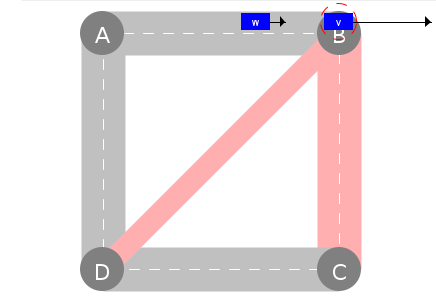
\includegraphics[scale=0.35]{../../events/vehicle-at-intersection-before.png}
		\caption{Vehicle arrives at intersection.}
		\label{fig:vehicle-at-intersection-before}
	\end{subfigure}
	\begin{subfigure}{.45\textwidth}
		\centering
		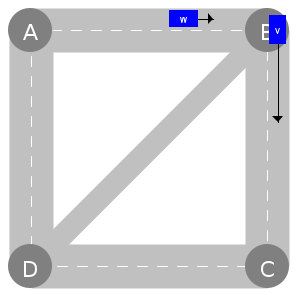
\includegraphics[scale=0.35]{../../events/vehicle-at-intersection-after.png}
		\caption{Vehicle departs at intersection.}
		\label{fig:vehicle-at-intersection-after}
	\end{subfigure}
	\caption{Vehicle-intersection location events.}
	\label{fig:routing-events}
\end{figure}

%\vspace{2mm}
\noindent \textbf{Vehicle arrives at intersection} (see Figure \ref{fig:vehicle-at-intersection-before}) occurs at time $t \in \mathbb{T}$ if and only if there exists a vehicle $v \in V$ and a location $(s,d) \in L$ with segment $s \in S$ and traveled distance $d \in \mathbb{R}_0^+$ such that the vehicle $v$ at time $t$ is at location $(s,d)$, i.e. $S_{V.CL}(v,t) = (s,d)$, and the traveled distance $d$ on segment $s$ equals the length of the segment $s$, i.e. $P_{S.L}(s) = d$.

\vspace{2mm}
\noindent \textbf{Vehicle departs at intersection} (see Figure \ref{fig:vehicle-at-intersection-after}) occurs at time $t \in \mathbb{T}$ if and only if there exists a vehicle $v \in V$ and a location $(s,d) \in L$ with segment $s \in S$ and traveled distance $d \in \mathbb{R}_0^+$ such that the vehicle $v$ at time $t$ is at location $(s,d)$, i.e. $S_{V.CL}(v,t) = (s,d)$, and the traveled distance $d$ on segment $s$ is zero, i.e. $d = 0$.

\vspace{2mm}
\noindent \textit{Note that each vehicle arrives at intersection event occurs concurrently with a follow-up vehicle departs at intersection event.}

\subsection{Vehicle-charging station location events}
\label{sec:charging-station-location-events}

Vehicle-charging station events occur, when vehicles arrive at charging stations.
These events have been included in the formalism, because vehicles need to make charging decisions when arriving at charging stations. 

\vspace{2mm}
\noindent \textbf{Vehicle arrives at charging station} occurs at time $t \in \mathbb{T}$ if and only if there exists a vehicle $v \in V$ and a charging station $cs \in CS$ with location $l = P_{CS.L}(cs)$, such that the vehicle $v$ at time $t$ is at location $l$, i.e. $S_{V.CL}(v, t) = l$, and for all previous times $t' \in \mathbb{T}$ with $t' < t$ where vehicle $v$ was at location $l$, i.e. $S_{V.CL}(v, t') = l$, there exists an intermediate time $t'' \in \mathbb{T}$ with $t' < t'' < t$, such that vehicle $v$ was not at location $l$, i.e. $S_{V.CL}(v, t'') \neq l$.

\subsubsection{Vehicle-demand location events}
\label{sec:demand-location-events}

Vehicle-demand location events occur, when vehicles arrive at demand pick-up and drop-off locations (see Figure~\ref{fig:demand-events}).
These events have been included in the formalism, because vehicles need to make demand pick-up decisions and perform drop-offs.

\begin{figure}[htbp]
    \centering
	\begin{subfigure}{.45\textwidth}
		\centering
		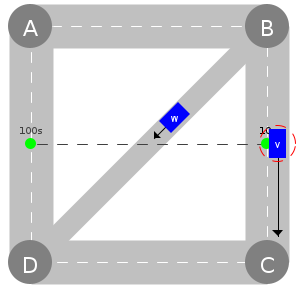
\includegraphics[scale=0.35]{../../events/vehicle-at-demand-pick-up.png}
		\caption{Vehicle at demand pick-up.}
		\label{fig:vehicle-at-demand-pick-up}
	\end{subfigure}
	\begin{subfigure}{.45\textwidth}
		\centering
		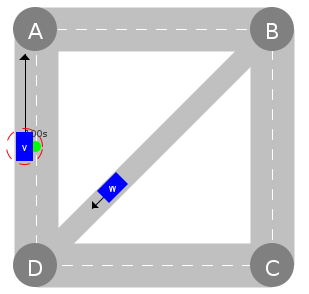
\includegraphics[scale=0.35]{../../events/vehicle-at-demand-drop-off.png}
		\caption{Vehicle at demand drop-off.}
		\label{fig:vehicle-at-demand-drop-off}
	\end{subfigure}
	\caption{Vehicle-demand location events.}
	\label{fig:demand-events}	
\end{figure}

%\vspace{2mm}
\noindent \textbf{Vehicle arrives at demand pick-up location} (see Figure \ref{fig:vehicle-at-demand-pick-up}) occurs at time $t \in \mathbb{T}$ if and only if there exists a vehicle $v \in V$ and a demand $d \in D$ with demand pick-up location $pl = P_{D.PL}(d)$, such that the vehicle $v$ at time $t$ is at demand pick-up location $pl$, i.e. $S_{V.CL}(v, t) = pl$, and for all previous times $t' \in \mathbb{T}$ with $t' < t$ where vehicle $v$ was at demand pickup location $pl$, i.e. $S_{V.CL}(v, t') = pl$, there exists an intermediate time $t'' \in \mathbb{T}$ with $t' < t'' < t$, such that vehicle $v$ was not at demand pick-up location $pl$, i.e. $S_{V.CL}(v, t'') \neq pl$.

\vspace{2mm}
\noindent \textbf{Vehicle arrives at demand drop-off location} (see Figure \ref{fig:vehicle-at-demand-drop-off}) occurs at time $t \in \mathbb{T}$ if and only if there exists a vehicle $v \in V$ and a demand $d \in D$ with demand drop-off location $dl = P_{D.DL}(d)$, such that the vehicle $v$ at time $t$ is at demand drop-off location $dl$, i.e. $S_{V.CL}(v, t) = dl$, and for all previous times $t' \in \mathbb{T}$ with $t' < t$ where vehicle $v$ was at demand drop-off location $dl$, i.e. $S_{V.CL}(v, t') = dl$, there exists an intermediate time $t'' \in \mathbb{T}$ with $t' < t'' < t$, such that vehicle $v$ was not at demand drop-off location $dl$, i.e. $S_{V.CL}(v, t'') \neq dl$.

\subsubsection{Vehicle-vehicle location events}
\label{sec:vehicle-location-events}

Vehicle-vehicle location events occur, when a vehicle starts and finishes overtaking another vehicle (see Figure~\ref{fig:overtaking-events}).
These events have been included in the formalism, because there needs to be enough space for vehicles overtaking each other. 

\begin{figure}[htbp]
	\centering
	\begin{subfigure}{.45\textwidth}
        \centering
        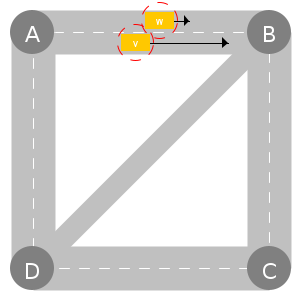
\includegraphics[scale=0.35]{../../events/faster-vehicle-front-at-slower-vehicle-back.png}
        \caption{Faster vehicle arrives at slower vehicle}
        \label{fig:faster-vehicle-front-at-slower-vehicle-back}
	\end{subfigure}
	\begin{subfigure}{.45\textwidth}
        \centering
        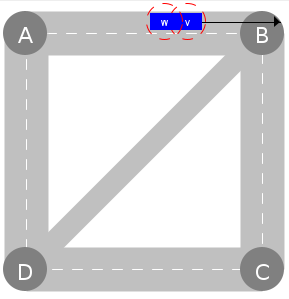
\includegraphics[scale=0.35]{../../events/slower-vehicle-front-at-faster-vehicle-back.png}
        \caption{Faster vehicle departs at slower vehicle}
        \label{fig:slower-vehicle-front-at-faster-vehicle-back}
	\end{subfigure}
	\caption{Vehicle-vehicle location events.}
	\label{fig:overtaking-events}
\end{figure}

%\vspace{2mm}
\noindent \textbf{Faster vehicle arrives at slower vehicle} (see Figure \ref{fig:faster-vehicle-front-at-slower-vehicle-back}) occurs at time $t \in \mathbb{T}$ if and only if there exists a faster vehicle $v_{f} \in V$ and a slower vehicle $v_{s} \in V$ with current locations $(s_f, d_f) = S_{V.CL}(v_f, t)$ and $(s_s, d_s) = S_{V.CL}(v_s, t)$, such that the current driving speed of the faster vehicle $v_f$ is greater than the current driving speed of the slower vehicle $v_s$, i.e.\ $S_{V.CDS}(v_f, t) > S_{V.CDS}(v_s, t)$, the segment $s_f$ of the faster vehicle $v_f$ is equal to the segment $s_s$ of the slower vehicle $v_s$, i.e.\ $s_f = s_s$, and the distance $d_f$ plus half the vehicle length $l_f$ of the faster vehicle $v_f$ equals the distance $d_s$ minus half the vehicle length $l_s$ of the slower vehicle $v_s$, i.e.\ $d_f + l_f / 2 = d_s - l_s / 2$.

\vspace{2mm}
\noindent \textbf{Faster vehicle departs at slower vehicle} (see Figure \ref{fig:slower-vehicle-front-at-faster-vehicle-back}) occurs at time $t \in \mathbb{T}$ if and only if there exists a faster vehicle $v_{f} \in V$ and a slower vehicle $v_{s} \in V$ with current locations $(s_f, d_f) = S_{V.CL}(v_f, t)$ and $(s_s, d_s) = S_{V.CL}(v_s, t)$, such that the current driving speed of the faster vehicle $v_f$ is greater than the current driving speed of the slower vehicle $v_s$, i.e.\ $S_{V.CDS}(v_f, t) > S_{V.CDS}(v_s, t)$, the segment $s_f$ of the faster vehicle $v_f$ is equal to the segment $s_s$ of the slower vehicle $v_s$, i.e.\ $s_f = s_s$, and the distance $d_f$ minus half the vehicle length $l_f$ of the faster vehicle $v_f$ equals the distance $d_s$ plus half the vehicle length $l_s$ of the slower vehicle $v_s$, i.e.\ $d_f - l_f / 2 = d_s + l_s / 2$.

\subsection{Demand events}
\label{sec:demand-events}

Demand events occur, when the information about demands appears in the computer simulation.
This event has been included in the formalism, because when information about demands appears the vehicles can change their behavior.

\vspace{2mm}
\noindent \textbf{Demand appears} occurs at time $t \in \mathbb{T}$ if and only if there exists a vehicle $v \in V$ and a demand $d \in D$, such that the demand $d$ at time $t$ doesn't have an assigned current vehicle $v$, i.e. $S_{D.CV}(d, t) = \{\perp\}$, and such that the demands appear time $P_{D.AT}$ equals the current time $t$, i.e. $P_{D.AT} = t$.

\subsection{Speed events}
\label{sec:speed-events}

Speed events occur, when vehicles change their driving and charging speeds.
These events have been included in the formalism, because drive speeds influence overtaking behaviors and charging speeds influence electric loads.

\vspace{2mm}
\noindent \textbf{Vehicle drive speed changes} occurs at time $t \in \mathbb{T}$ if and only if there exists a vehicle $v \in V$ with current drive speed $S_{V.CDS}(v, t)$, such that for all previous times $t' \in \mathbb{T}$ with $t' < t$, where the current drive speed $S_{V.CDS}(v,t')$ of vehicle $v$ at time $t'$ was identical, i.e. $S_{V.CDS}(v,t') = S_{V.CDS}(v,t)$, there exists an intermediate time $t'' \in \mathbb{T}$ with $t' < t'' < t$, such that the current drive speed $S_{V.CDS}(v,t'')$ of vehicle $v$ at time $t''$ is different, i.e. $S_{V.CDS}(v,t'') \neq S_{V.CDS}(v,t)$.

\vspace{2mm}
\noindent \textbf{Vehicle charge speed changes} occurs at time $t \in \mathbb{T}$ if and only if there exists a vehicle $v \in V$ with current charge speed $S_{V.CCS}(v, t)$, such that for all previous times $t' \in \mathbb{T}$ with $t' < t$, where the current charge speed $S_{V.CCS}(v,t')$ of vehicle $v$ at time $t'$ was identical, i.e. $S_{V.CCS}(v,t') = S_{V.CCS}(v,t)$, there exists an intermediate time $t'' \in \mathbb{T}$ with $t' < t'' < t$, such that the current charge speed $S_{V.CCS}(v,t'')$ of vehicle $v$ at time $t''$ is different, i.e. $S_{V.CCS}(v,t'') \neq S_{V.CCS}(v,t)$.


\subsection{Battery events}
\label{sec:battery-events}

Battery events occur, when the vehicle batteries are either empty or full.
These events have been included in the formalism, because vehicles with empty batteries stop driving and vehicles with full batteries stop charging.

\vspace{2mm}
\noindent \textbf{Vehicle battery becomes empty} occurs at time $t \in \mathbb{T}$ if and only if there exists a vehicle $v \in V$ such that the current battery level of vehicle $v$ at time $t$ is zero, i.e. $S_{V.CBL}(v,t) = 0$ and for all previous times $t' \in \mathbb{T}$ with $t' < t$, where the current battery level of vehicle $v$ was zero, i.e. $S_{V.CBL}(v,t') = 0$, there exists an intermediate time $t'' \in \mathbb{T}$ with $t' < t'' < t$, such that the current battery level of vehicle $v$ was not zero, i.e. $S_{V.CBL}(v,t'') \neq 0$.

\vspace{2mm}
\noindent \textbf{Vehicle battery becomes full} occurs at time $t \in \mathbb{T}$ if and only if there exists a vehicle $v \in V$ such that the current battery level of vehicle $v$ at time $t$ equals the maximum battery level of vehicle $v$, i.e. $S_{V.CBL}(v,t) = P_{V.MBL}(v)$, and for all previous times $t' \in \mathbb{T}$ with $t' < t$, where the current battery level of vehicle $v$ equals the maximum battery level of vehicle $v$, i.e. $S_{V.CBL}(v,t') = P_{V.MBL}(v)$, there exists an intermediate time $t'' \in \mathbb{T}$ with $t' < t'' < t$, such that the current battery level of vehicle $v$ does not equal the maximum battery level of vehicle $v$, i.e. $S_{V.CBL}(v,t'') \neq P_{V.MBL}(v)$.

\section{Conclusion}
\label{sec:con}

In this work, we presented a discrete event formalism for fast simulation of on-demand transportation systems. Our proposed formalization allows for reduction of simulation complexity by defining domain relevant events impacting the design problem at hand, while omitting unimportant details negatively impacting simulation performance, thereby reducing both modeling as well as simulation effort. In addition, the provided formalization of system theory and discrete events serves as an interface for deriving well-defined system structure as well as efficient control strategies. 
In terms of applicability and feasibility of the proposed approach, initial results show that it works well in scenarios, where cars are assumed to drive with constant speed most of the time as states can be omitted.
This assumption currently limits the validity of the model, because in real world conditions, car speeds may not always be constant.
However, we believe that this simplification provides sufficient validity for use cases such as transportation system and control strategy design.

\newpage
\bibliographystyle{plain}
\bibliography{main}

\end{document}